%!TEX ROOT=../diploma-thesis.tex

\chapter{Rešerše}\label{ch:reserse}

Tato kapitola se věnuje rešerši existujících řešení
a výzkumu relevantnímu k tématu této práce. Díky tomu bude umožněno
dosáhnout kvalitního a efektivního návrhu frameworku pro centrální správu a automatickou
distribuci byznysových pravidel.

\section{Modelem ř\'{\i}zená architektura}

Modelem řízená architektura (\gls{MDA} z anglického \textit{Model-Driven
Architecture}) se zaměřuje na návrh \gls{EIS} s využitím modelů a jejich
následnou transformaci do spustitelného kódu pomocí generativních nástrojů~\cite{soley2000model}.
Hlavní výhodou \gls{MDA} je vysoká úroveň abstrakce, která zbavuje vývojáře nutnosti
manuálně duplikovat informace. Další výhodou je nezávislost na platformě a zvýšení
kvality kódu díky jeho automatickému generování.

\gls{MDA} v první fázi vývoje využívá Computation Independent Model (\gls{CIM}), který reprezentuje
řešení nezávislé na použitých výpočetních metodách a algoritmech. Z \gls{CIM} je
následně model převeden do Platform Independent Model (\gls{PIM}),
který popisuje koncepci systému bez ohledu na implementační detaily, typicky k popisu
využívá jazyk \gls{UML}. \gls{PIM} je následně převeden do
Platform Specific Model (\gls{PSM}), tedy do modelu využívajícího
specifických aspektů platformy, pro kterou má být systém postaven.
\gls{PIM} může být převeden na jeden či více \gls{PSM}.
Nakonec je \gls{PSM} transformován do spustitelného kódu~\cite{kleppe2003model}.

Hlavní nevýhodou \gls{MDA}, která zabraňuje jejímu využití
pro účel této práce, je jednosměrný dopředný proces, kterým je výsledný kód generován.
Pokud dojde ke změně požadavků, která se promítne do modelu, je potřeba přegenerovat
kód celého systému. Kód, který bylo nutno doplnit ručně, může snadno zastarat a je tak
potřeba ho manuálně projít a opravit.
Další nevýhodou tohoto přístupu je jeho závislost na \gls{OOP},
které samotné není schopné se efektivně vypořádat s průřezovými
problémy~\cite{kennard2009separation}\cite{cemus2014aspect},
jak bude demonstrováno v sekci~\ref{sec:aop}.

\section{Generativní programování}

Generativní programování (\gls{GP}) je dalším příkladem paradigmatu, který
využívá vyšší úroveň abstrakce a díky tomu zvyšuje znovupoužitelnost
kódu. \gls{GP} se zaměřuje na maximalizaci automatizace vývoje systému
skrz generování a syntézu vysoce přizpůsobitelných komponent. Vývojář
popíše komponentu v abstraktním jazyce přizpůsobeném doméně řešeného
problému a generátor se postará o její automatické vytvoření~\cite{czarnecki2000generative}.
Díky tomu je možné oddělit popis jednotlivých vlastností systému a dosáhnout tak
jejich vysoké znovupoužitelnosti.

\gls{GP} by mohlo být využito pro abstrakci bynysových pravidel a jejich automatickému
začleňování do kódu služeb v systému stavějícím na \gls{SOA}.
Statické generování komponent však nesplňuje požadavek na dynamickou správu
byznysových pravidel za běhu systému.

\section{Metaprogramování}

Metaprogramování je alternativním paradigmatem, které vnímá kód programu
zároveň jako data, se kterými program může pracovat. To programu umožňuje
číst, vytvářet či upravovat jiné programy včetně sama sebe. Tyto činnosti
lze provádět staticky, ale i za běhu daného programu~\cite{sheard2001accomplishments}\cite{czarnecki2000generative}.
Program, který manipuluje s kódem, se nazývá \textit{metaprogram}. Programovací
jazyk, který umožňuje programování, se nazývá \textit{metajazyk} (z anglického
\textit{metalanguage})~\cite{visser2002meta}. Schopnost programovacího jazyka
být sám sobě metajazykem se nazývá \textit{reflexe}~\cite{sobel1996introduction}.

Tento přístup přináší vysokou úroveň abstrakce a zvýšenou efektivitu
vývojářů, kteří jsou schopni automaticky provádět inspekci, generovat a upravovat
programy. Reflexe je součástí moderních programovacích jazyků a je
využívána mnoha frameworky a knihovnami~\cite{vandevoorde2002c++}~\cite{forman2004java}.
Jedním z vhodných využití metaprogramování je implementace \gls{DSL}~\cite{sheard2001accomplishments}.

\section{Business Process Execution Language}

Technologie Business Process Execution Language (\gls{BPEL}) využívá speciálního \gls{DSL}
postaveného na jazyku \gls{XML} k popisu byznysových procesů realizovaných webovými
službami~\cite{andrews2003business}. Umožňuje \textit{top-down} realizaci \gls{SOA}
skrz kompozici, orchestraci a koordinaci služeb~\cite{oraclebpel}.
Přístup \gls{BPEL} využívá meta-služby, které se starají o uložení a transformaci byznysových pravidel
a také o zachycení byznysových operací a aplikaci těchto pravidel~\cite{rosenberg2005business}.

\gls{BPEL} přináší možnost využít byznysová pravidla spravovaná doménovými experty
v procesně orientovaném prostředí \gls{SOA}. Díky tomu výrazně zvyšuje kvalitu a snižuje
náročnost vývoje. Nejnovější výzkum v oblasti \gls{SOA} a zejména Microservices
však od orchestrace ustupuje na úkor decentralizace a choreografie
služeb~\cite{bakshi2017microservices}\cite{cerny2018contextual}.

\section{Objektově orientované programování}\label{sec:oop}

%\goal{OOP a jeho popis}
Jedn\'{\i}m z nejpoužívanějších paradigmat používaných k
v\'yvoji modern\'{\i}ch \gls{EIS} je objektově orientované programován\'{\i} (\gls{OOP}).
To používá koncept tzv. objektů, které zapouzdřují data a funkcionalitu do
malých funkčních celků odpov\'{\i}daj\'{\i}c\'{\i} struktuře reálného světa~\cite{rentsch1982object}.
Objekty se rozum\'{\i} jak konkrétn\'{\i} koncepty, např\'{\i}klad auto nebo člověk, tak i
abstraktn\'{\i} koncepty, jako je bankovn\'{\i} transakce nebo objednávka v obchodě.
Podoba objektů se pak prom\'{\i}tá do kódu programu i do reprezentace struktur v paměti
poč\'{\i}tače. Tento př\'{\i}stup je velmi snadn\'y pro pochopen\'{\i},
vede k lepš\'{\i}mu návrhu a organizaci programu a snižuje
tak náklady na jeho v\'yvoj a údržbu.

Vlastnosti \gls{OOP}, jako je zapouzdření, dědičnost a polymorfismus, přináší
vysokou znovupoužitelnost kódu, nižší riziko lidské chyby, zjednodušení
návrhu systému a nižší náklady na vývoj a údržbu software.

\section{Aspektově orientované programován\'{\i}}\label{sec:aop}

\subsection{Motivace}

%\goal{Nedostatky OOP}
Ačkoliv je \gls{OOP} velmi siln\'ym nástrojem, existuj\'{\i} problémy,
které nelze v jeho rámci efektivně řešit.
Příkladem takového problému jsou obecné požadavky na systém,
které musej\'{\i} b\'yt konzistentně dodržovány na v\'{\i}ce
m\'{\i}stech systému, které spolu zdánlivě nesouvis\'{\i},
tzv. \textit{průřezové problémy} (z anglického \textit{cross-cutting concerns}).
V rámci \gls{OOP} je programátor nucen v ojektech manuálně opakovat
kód, kter\'y zodpov\'{\i}dá za jejich realizaci. Duplikace kódu
vede k větš\'{\i} náchylnosti na lidskou chybu a k vyšš\'{\i}m nárokům na v\'yvoj
a údržbu daného softwarového systému~\cite{fowler1999refactoring}.
Obrázek~\ref{fig:cross-cutting} znázorňuje vzájemné postavení průřezových
problémů a komponent informačního systému.

\begin{figure}[t]
    \centering
    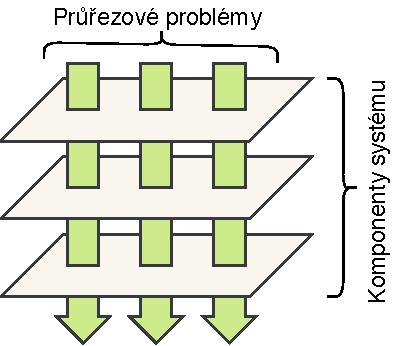
\includegraphics[keepaspectratio=true, width=0.35\linewidth]{figures/cross-cutting.pdf}
    \caption{Průřezové problémy v informačních systémech}
    \label{fig:cross-cutting}
\end{figure}

\begin{definition}
    Průřezový problém je vlastnost systému, která ovlivňuje více jeho komponent
    zásahem do jejich funkcionality~\cite{kiczales1997aspect}.
\end{definition}

%\goal{Konkrétní příklad nedostatku OOP}
Př\'{\i}kladem průřezového problému může b\'yt logován\'{\i}
systémov\'ych akc\'{\i}, optimalizace správy paměti
nebo jednotné zpracován\'{\i} v\'yjimek~\cite{kiczales1997aspect},
ale i aplikace byznysových pravidel~\cite{cemus2014aspect}.
Ve zdrojovém kódu~\ref{lst:tangling} je znázorněno, jak průřezové
problémy zasahují do kódu imaginární třídy implementované v
jazyce Java, která slouží pro vytváření objednávek v e-commerce
systému popsaném v sekci~\ref{sec:shortcomings}.
Aspekt logování je zohledněn na třech místech, stejně jako aspekt transakcí.
Navíc jsou zde zohledněna i byznysová pravidla pro validaci doručovací
a fakturační adresy objednávky.

\lstinputlisting[
caption={Příklad průřezových problémů zohledněných při vytváření objednávky},
label={lst:tangling},
language=Java,
float,
floatplacement=t
]
{code/tangling.java}

\subsection{Vlastnosti}
Aspektově orientované programován\'{\i} (\gls{AOP}) přináš\'{\i} řešen\'{\i}
v\'yše zmiňovaných problémů. Využívá k tomu \textit{separation of concerns} \textendash\xspace
extrahuje kód zachycující průřezové problémy, tzv. \textit{aspekty}, do jednoho bodu, tzv. (\textit{single focal point}).
Pomoc\'{\i} procesu zvaného \textit{weaving} je poté tento kód automaticky distribuován.
Weaving může proběhnout staticky při kompilaci programu nebo dynamicky
při jeho běhu. V obou př\'{\i}padech ale programátorovi ulehčuje práci,
protože k definici i změně aspektu docház\'{\i} centrálně, a t\'{\i}m je eliminována
potřeba manuáln\'{\i} duplikace kódu. \gls{AOP} nen\'{\i} paradigmatem poskytuj\'{\i}c\'{\i}m
kompletn\'{\i} framework pro návrh programu. V ideáln\'{\i}m př\'{\i}padě je tedy k návrhu
systému využita kombinace \gls{AOP} s jin\'ym paradigmatem.

\subsection{Názvosloví}

%\paragraph{Aspekt}
Základním pojmem v rámci \gls{AOP} je \textit{aspekt},
který zapozdřuje průřezovou funkcionalitu a zároveň adresuje místa, kde má být
funkcionalita aplikována. Aspekt vždy obsahuje alespoň jeden \textit{advice}
a jeden \textit{pointcut}.

%\paragraph{Join-point}
Místo v kódu, na které může být aplikována funkcionalita aspektu, se nazývá
\textit{join-point}. Typů join-pointů je více a závisí na použitém paradigmatu,
na který je \gls{AOP} aplikováno, a také na programovacím jazyce. V případě
kombinace s \gls{OOP} a klasickým víceúčelovým jazykem jako je například Java,
mohou jako join-pointy sloužit konstruktory tříd, volání metod, zápis a čtení
z atributu objektu, inicializace třídy nebo objektu a mnoho dalších.

%\paragraph{Pointcut}
Množina join-pointů, na které je jeden konkrétní aspekt aplikován, se nazývá \textit{pointcut}.
Tato množina může být určena staticky, a být tak známá při kompilaci programu, nebo
dynamicky za běhu programu, což přináší výpočetní složitost navíc výměnou
za vyšší flexibilitu.

%\paragraph{Advice}
Funkcionalita, kterou aspekt přidává v jeho pointcutu, se nazývá
\textit{advice}. Existuje více typů advice, podle toho, kam je
daná funkcionalita přidána. Například při volání metody může
být funkcionalita přidána před, za, nebo kolem metody.

%\paragraph{Weaving}
Proces, kterým jsou advice začleňovány podle pointcutu do
jednotlivých join-pointů se nazývá \textit{weaving}. Ten může
probíhat již při kompilaci nebo dynamicky za běhu programu,
tzv. \textit{run-time weaving}. Proces weavingu je ilustrován
na obrázku~\ref{fig:aspect-weaving}. Komponenta zodpovědná za
weaving se nazývá \textit{aspect weaver}.

\begin{figure}[t]
    \centering
    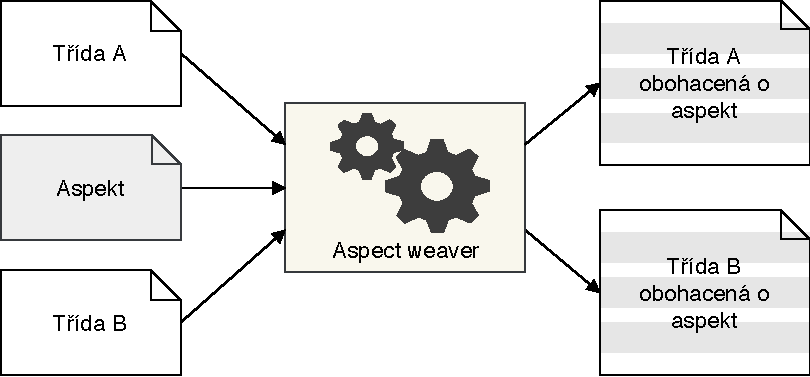
\includegraphics[keepaspectratio=true, width=0.7\linewidth]{figures/aspect-weaving.pdf}
    \caption{Proces weavingu aspektů}
    \label{fig:aspect-weaving}
\end{figure}

\section{Aspect-driven Design Approach}\label{sec:adda}

\subsection{Vlastnosti}

Alternativním způsobem návrhu informačních systémů, který staví na principech \gls{AOP},
je Aspect-driven Design Approach\footnote{Autoři nejprve používali termín \textit{Aspect-Oriented
Design Approach} (AODA), který byl později změněn. Oba tyto pojmy jsou vzájemně zaměnitelné.}
(\gls{ADDA})~\cite{cemus2014aspect}, představený v roce 2014.
Tento přístup se zaměřuje na formalizaci jednotlivých komponent informačních systémů identifikování aspektů
v informačních systémech a jejich separaci do \textit{single focal point}.
Následně přístup využívá weaving pro automatickou distribuci aspektů do systému.
K popisu aspektu doporučuje využití doménově specifického jazyka, který bude navržen na
míru danému průřezovému problému.

\subsection{Možnosti aplikace}

Autoři \gls{ADDA} aplikovali tento koncept v několika oblastech \gls{EIS}.
Mezi tyto oblasti patří automatické začleňování byznysových pravidel
do datové vrstvy informačních systémů~\cite{cemus2015automated}, automatické
generování uživatelských rozhraní citlivých na kontext uživatele~\cite{cemus2017separation},
validaci vstupů formulářů v uživatelském rozhraní vůči byznysovým pravidlům~\cite{cemus2016context}\cite{cemus2017separation}
a automatické extrakci dokumentace~\cite{cemus2017automated}.

Jednou z možných aplikací přístupu \gls{ADDA} je automatické začleňování
byznysových pravidel do datové vrstvy \gls{EIS}\footnote{Předpokládáme standardní
třívrstvou architekturu informačních systémů~\cite{fowler2002patterns}}.
Byznysová pravidla jsou nejprve vhodně popsána pomocí \gls{DSL} a následně jsou
extrahována do jednoho bodu, ze kterého jsou automaticky distribuována.
Pomocí specializovaného weaveru jsou pravidla překládána do podmínek
jazyka \gls{JPQL}, potažmo \gls{SQL}, který je využíván k získávání dat
z databázových systémů. To vede ke snížení manuální duplikace byznysových
pravidel.

Uživatelská rozhraní tvoří až 48 \% kódu informačních systému
a zabírají až 50 \% jejich vývojového času~\cite{kennard2009separation}.
Do \gls{UI} se přitom typicky promítá mnoho aspektů, které jsou
již v systému obsaženy. Například byznysová pravidla jsou promítána do \gls{UI}
při validaci vstupních dat formulářů na straně klienta~\cite{cemus2017separation}.
Autoři přístupu \gls{ADDA} přicházejí s řešením v podobě
využití několika \gls{DSL} pro popis jednotlivých aspektů
a run-time weavingu, který aspekty při běhu aplikace
dynamicky začlení do \gls{UI} s ohledem na aktuální kontext
uživatele, například na jeho geolokační polohu či velikost
displeje, na kterém je rozhraní zobrazováno.
Díky tomu je dosaženo významné redukce kódu~\cite{cemus2016context}
potřebného pro popis adaptibilního uživatelského rozhraní.

Další oblastí informačních systému, do které se promítají jeho aspekty,
je dokumentace~\cite{cemus2017automated}. Autoři \gls{ADDA}
využívají data mining pro získání metainformací o byznysových operacích,
datovém modelu systému a o byznysových pravidlech. Díky tomu mohou
automaticky vygenerovat seznam byznysových operací, potažmo implementovaných
use-cases, strukturu doménového modelu a formální popis byznysových pravidel,
který může sloužit pro verifikaci jejich správnosti.

\subsection{Výhody a nevýhody}

\gls{ADDA} poskytuje vývojářům způsob jakým výrazně snížit náklady na vývoj a údržbu
systému díky deduplikaci, která je dosažena extrakcí aspektů
do \textit{single focal point} a jejich automatickou distribucí do
příslušných komponent systému. Tento přístup však nese vysokou počáteční investici v
podobě vývoje specializovaných \gls{DSL} a dynamických aspect weaverů.
Ačkoliv autoři tohoto přístupu implementovali prototypy knihoven umožňující
požadovanou funkcionalitu, pro nasazení do reálného systému
nejsou tyto knihovny připraveny.

Přístup \gls{ADDA} splňuje požadavky identifikované v sekci~\ref{sec:implementation-requirements},
zejména využití speciálních \gls{DSL} pro popis aspektů a
jejich automatickou distribuci za běhu systému. Pro popis byznysových pravidel
využívá \gls{ADDA} nástroj \textit{Drools}, který je popsán v následující sekci.

\section{Stávaj\'{\i}c\'{\i} řešen\'{\i} reprezentace business pravidel}\label{sec:business-rule-dsl}

Tato kapitola se zaměřuje i na současné možnosti zachycení
byznysových pravidel ve specializovaných jazycích a vhodnost jejich použití
pro účel frameworku, který bude výstupem této práce.
Ačkoliv existuje relativně velké množství knihoven poskytujících
\gls{DSL} pro popis byznysových pravidel a umožňující automatickou
distribuci byznys pravidel, žádný z nich nepodporuje dostatečně velké množství
platforem, ve kterých by mohl být jazyk použit. Příkladem může být projekt \textit{business-ruless}
pro jazyk Python\footnote{https://pypi.org/project/business-rules/}, projekt
FlexRule\footnote{http://www.flexrule.com/archives/business-rule-language/} pro platformy .NET a
JavaScript nebo \gls{BRMS} JRules~\cite{boyer2011ibm} od společnosti \gls{IBM} pro platformu \gls{Java EE}.
Tato sekce se proto zaměřuje zejména na framework Drools, který používají autoři přístupu \gls{ADDA},
a také na moderní nástroj JetBrains MPS, který umožňuje vytvářet vlastní \gls{DSL} a transformovat
ho do dalších jazyků.

\begin{definition}
    \gls{DSL} je programovací jazyk určený k popisu specifické vlastnosti či funkce systému v
    rámci dané domény~\cite{fowler2010domain}.
\end{definition}

\subsection{Drools DSL}\label{sec:drools}

Framework Drools\footnote{https://www.drools.org/} je open-source projekt realizující
\textit{business rule management engine} (\gls{BRMS}), tedy nástroj pro vývoj a správu byznysových
pravidel. Framework umožňuje vývoj tzv. \textit{produkčních systémů} tvořených sadou \textit{produkčních pravidel}.
Produkční pravidlo se skládá z levé strany (\gls{LHS} z anglického \textit{left-hand side}),
a z pravé strany (\gls{RHS} z anglického \textit{right-hand side}).
\gls{LHS} popisuje situaci, při které má být pravidlo aplikováno. \gls{RHS} popisuje akci,
která má být vykonána. Pro určení produkčních pravidel, která mají být aplikována, je využit
algoritmus RETE~\cite{forgy1988rete}.

Součástí frameworku Drools je speciální doménově specifický jazyk vyvinutý přímo
pro modelování produkčních pravidel. Tento jazyk umožňuje popsat \gls{LHS} i \gls{RHS}
daného pravidla včetně zápisu logických výrazů, využití lokálních i globálních proměnných
s plnou typovou kontrolou a podporu regulárních výrazů. Navíc je možno importovat i pomocné funkce, které lze
využít v podmínkách pravidla.

Ačkoliv je jazyk Drools \gls{DSL} vymodelovaný přímo pro zápis pravidel doménovými experty,
produkční pravidla se liší od byznysových pravidel zavedených v sekci~\ref{sec:business-rules},
Využít tak lze pouze \gls{LHS}. Zároveň jazyk Drools \gls{DSL} postrádá
nástroje pro kvalitní popis byznysového kontextu držícího byznysová pravidla,
zejména pak rozšiřování jiných kontextů a popis typu jednotlivých pravidel~\cite{cemus2017automated}.
Ze strany frameworku Drools navíc nejsou podporovány jiné platformy než Java a .NET, což nevyhovuje
požadavkům na platformovou nezávislost.

\subsection{JetBrains MPS}

Moderním nástrojem pro tvorbu doménově specifických jazyků
je \textit{JetBrains MPS} (Meta Programming System)\footnote{https://www.jetbrains.com/mps/}.
Staví na konceptu \textit{language-oriented programming} (\gls{LOP})~\cite{ward1994language} zaměřujícího
se na vývoj specifického abstraktního jazyka a jeho použití pro implementaci programu. Pro překlad ze specifického
jazyka do spustitelného kódu je použit automatický překladač. Příkladem jazyka, který využívá koncept \gls{LOP}
je \LaTeX\xspace, který byl využit pro sazbu této diplomové práce. Ten totiž pomocí maker jazyka \TeX\xspace
sestavuje abstraktnější jazyk, který umožňuje autorovi soustředit se hlavně na strukturu textu, aniž by
se musel příliš detailně zaobírat samotnou sazbou.

MPS umožňuje uživateli nadefinovat gramatiku speciálního \gls{DSL} a následně poskytuje
editor pro tento jazyk včetně automatického validátoru. MPS také umožňuje transformování
nadefinovaného jazyka do obecných programovacích jazyků, zejména pak do jazyka Java.
Díky tomu lze nejen vytvářet libovolné \gls{DSL}, ale také rozšiřovat existující jazyky.

Výhoda tohoto přístupu je vysoká úroveň abstrakce a možnost zapojit do vývoje doménové experty.
\gls{DSL} zvyšuje expresivitu kódu a díky tomu se zmenšuje jeho objem.
Nižší objem kódu vede ke snížení nákladů na jeho údržbu a vývoj~\cite{littman1987mental}\cite{soloway1986empirical}.
Významnou výhodou MPS, potažmo \gls{LOP}, je nezávislost na cílové platformě.
Nástroj MPS by umožnil snadné znovupoužití pravidel a jejich transformaci do neomezeného počtu jazyků pro
využití na mnoha platformách. Podobně jako u \gls{MDA} je však problém v dopředném
generování \textendash\xspace editor MPS totiž neumožňuje načíst víceúčelový jazyk zpět do \gls{DSL}.

\section{Síťové architektury}

Závěrem se tato kapitola věnuje přehledu síťových architektur, které mohou být využity pro
distribuci byznysových pravidel v systému stavějícímu na \gls{SOA}.

\subsection{Architektura klient-server}\label{sec:client-server}

Model klient-server popisuje vztah mezi komponentami systému, klienty a serverem.
Klient zašle požadavek serveru a ten mu vrátí odpověď~\cite{berson1992client}.
Schéma komunikace je znázorněno na obrázku ~\ref{fig:client-server}.
Tento model může být použit obecně i v rámci jednoho počítače,
nejčastěji je však využíván v síťové komunikaci mezi více počítači.

\begin{figure}[t]
    \centering
    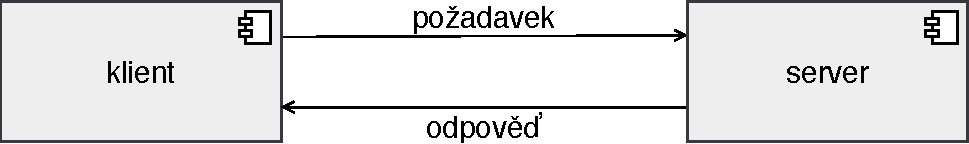
\includegraphics[keepaspectratio=true, width=0.6\linewidth]{figures/client-server.pdf}
    \caption{Architektura klient-server}
    \label{fig:client-server}
\end{figure}

Tento přístup má několik zásadních výhod, díky kterým se stal
široce využívaným. Díky svojí velmi obecné myšlence je nezávislý
na jakékoliv platformě.
Zároveň tato architektura přesouvá byznysovou logiku a
ukládání dat na server a díky tomu umožňuje
snadnější kontrolu nad systémem a jeho centrální administraci. S tím
je spojena i snažší škálovatelnost systému. V neposlední řadě
přináší model klient-server díky centralizaci i lepší zabezpečení,
kdy server může jasně definovat a vynucovat přístupová pravidla.

Hlavní nevýhodu této architektury je vytvoření jednoho centrálního bodu,
jehož výpadek ochromí funkci celého systému (v angličtině
\textit{single point of failure}) \textendash\xspace tímto bodem je server.
Pokud na serveru nastane chyba či výpadek, žádný z klientů není schopen využívat
jeho služeb.

\subsection{Architektura Peer-to-peer}\label{sec:p2p}

Opakem modelu klient-server je síťová architektura zvaná \textit{Peer-to-peer (\gls{P2P})}.
Jednotlivé počítače v síti spolu komunikují přímo, bez centrální autority.
Všechny počítače v síti jsou si vzájemně rovnocenné~\cite{fox2001peer}.
%Na obrázku~\ref{fig:peer-to-peer} je tato architektura znázorněna.
Hlavním cílem \gls{P2P} sítí je distribuce dat nebo výpočetních operací.

%\begin{figure}[t]
%    \centering
%    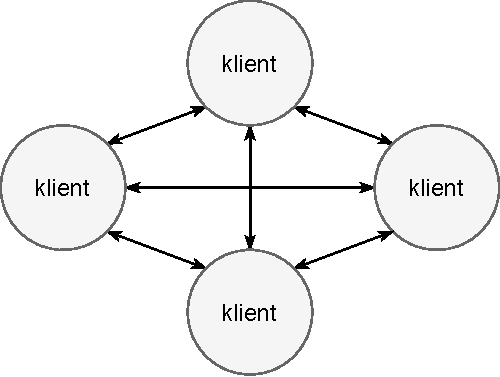
\includegraphics[keepaspectratio=true, width=0.4\linewidth]{figures/peer-to-peer.pdf}
%    \caption{Architektura peer-to-peer}
%    \label{fig:peer-to-peer}
%\end{figure}

Vysoká datová propustnost a robustnost \gls{P2P} by mohla být vhodná pro
sdílení byznysových pravidel. Absence centrální správy by však mohla způsobit
nekonzistenci při úpravě či přidání byznysového pravidla. Změna pravidla by se
musela šířit postupně napříč systémem, přičemž některé uzly by stále využívaly starou
verzi pravidla.

\subsection{Representational state transfer}\label{sec:rest}

Representational state transfer (\gls{REST}) je architektura
webových služeb, která staví na protokolu \gls{HTTP}, a klade na systém
několik architektonických omezení, díky kterým může systém dosáhnout
lepšího výkonu, vyšší škálovatelnosti, jednoduchému používání
a lepší odolnosti vůči chybám~\cite{fielding2000rest}. Principy architektury
\gls{REST} zahrnují využití architektury klient-server, bezestavovost a kešování požadavků,
vrsvení systému, zdrojový kód na vyžádání a jednotné rozhraní.
\gls{REST} modeluje systém jako množinu zdrojů (z anglického \textit{resources}),
nad kterými jsou prováděny operace pomocí \gls{HTTP} požadavků.

Nevýhodou architektury \gls{REST} je náročná implementace transakcí, které zahrnují více
zdrojů najednou. Protokol \gls{HTTP} nepodporuje uzavření více požadavků do jedné atomické
transakce. To může být problém v \gls{SOA} zejména pokud je vyžadována kooperace více služeb
najednou při vykonávání byznysové operace. Existují však koncepty, které využívají model
Try-Cancel/Confirm~\cite{pardon2011towards}, umožňující zajistit atomické transakce nad
\gls{REST} architekturou.

\subsection{Remote procedure call}\label{sec:rpc}

Architektura \gls{RPC} staví na modelu klient-server a umožňuje jednomu procesu (klientovi)
zavolat proceduru na druhém, vzdáleném procesu (serveru).
\gls{RPC} zapouzdřuje síťovou komunikaci a v programu samotném
je vzdálená procedura volána stejným způsobem jako lokální procedury~\cite{nelson1981remote}. Základním
prvkem architektury na klientovi i na serveru je tzv. \textit{stub}. Tato komponenta
umožňuje volat, resp. obsloužit, vzdálenou proceduru lokálně a zapozdřuje veškerou
síťovou komunikaci a serializaci či deserializaci argumentů, resp. návratových hodnot.

\section{Shrnut\'{\i}}

V této kapitole byla provedena rešerše architektur, paradigmat a frameworků, které by mohly být vhodné
pro řešení sdílení byznysových pravidel v \gls{SOA}, a shrnula jejich v\'yhody a nev\'yhody.
Nejvíce se kapitola věnovala inovativnímu přístupu k návrhu softwarov\'ych systémů \textit{ADDA},
ze kterého bude vycházet návrh frameworku, který bude výstupem této práce.
Kapitola také shrnula rešerši stávaj\'{\i}c\'{\i}ch řešen\'{\i} reprezentace byznys pravidel
a zhodnotila jejich vhodnost pro použití v této práci. Nakonec kapitola studovala existující
síťové architektury, které by mohly být využity pro distribuci byznysových pravidel v rámci \gls{SOA}.
